\documentclass[11pt,a4paper]{article}

% Marges du document %
\setlength{\topmargin}{0cm}
\setlength{\headheight}{0.4cm}
\setlength{\headsep}{0.8cm}
\setlength{\footskip}{1cm}
\setlength{\textwidth}{17cm}
\setlength{\textheight}{25cm}
\setlength{\voffset}{-1.5cm}
\setlength{\hoffset}{-0.5cm}
\setlength{\oddsidemargin}{0cm}
\setlength{\evensidemargin}{0cm}

\usepackage{amssymb}
\usepackage{psfrag}
\usepackage[utf8]{inputenc}
\usepackage[francais]{babel}
\usepackage[T1]{fontenc}
\usepackage{amsmath}
\usepackage{amsfonts}
\usepackage{amssymb}
\usepackage{graphicx}
\usepackage{subcaption}
\usepackage{fancyhdr}
\usepackage{multicol}
\usepackage{eurosym} % symbole €
\usepackage{siunitx}
\usepackage{stmaryrd}
\usepackage{bm}
\def\€{\euro{}}

\numberwithin{equation}{section}

\newcommand{\CC}{C\nolinebreak\hspace{-.05em}\raisebox{.4ex}{\tiny\bf +}\nolinebreak\hspace{-.10em}\raisebox{.4ex}{\tiny\bf +}}
\def\CC{{C\nolinebreak[4]\hspace{-.05em}\raisebox{.4ex}{\tiny\bf ++}}}

\newcommand\numberthis{\addtocounter{equation}{1}\tag{\theequation}} 

\usepackage{color} % gestion de différentes couleurs
\definecolor{linkcolor}{rgb}{0,0,0}
\definecolor{linkcolorurl}{rgb}{0,0,1}
\usepackage[ pdftex,colorlinks=true,
pdfstartview=FitV,
linkcolor= linkcolor,
citecolor= linkcolor,
urlcolor= linkcolorurl,
hyperindex=true,
hyperfigures=false]
{hyperref} % fichiers pdf 'intelligents', avec des liens entre les références, etc.

% En-tête et pied de page % 
\pagestyle{fancy}
\fancyhead[L]{\scriptsize \textsc{Titre}} 
\fancyhead[R]{\scriptsize \textsc{BUNEL Félix et VERGNET Hadrien}} 
\fancyfoot[C]{ \thepage}

\author{Bunel Félix et Vergnet Hadrien}

%%%%%%%%%%%%%%%%%%%%%%%%%%%%%
% Tikz packages and settings
%%%%%%%%%%%%%%%%%%%%%%%%%%%%%

\usepackage{tikz}
\usepackage{pgfplots}
\usepackage{tikz-3dplot}
\pgfplotsset{compat=1.11}

\usetikzlibrary{shapes.geometric,calc,intersections}
\usetikzlibrary{shapes.arrows}
\usetikzlibrary{shadings}
\usetikzlibrary{patterns}
\usetikzlibrary{decorations.pathmorphing}
\usetikzlibrary{decorations.pathreplacing}


\usetikzlibrary{external}
\tikzset{external/aux in dpth={false}}
\tikzset{external/up to date check={simple}}
\tikzset{external/optimize command away={\includetexgraphics}{2}}

\tikzset{>=stealth}

%%%%%%%%%%%%%%%%%%%%%%%%%%%%%%%%%%%%%%%%%%%%%%%%%%%%%%%%%%%%
% Custom macro to input a tikz picture and setting its name
%%%%%%%%%%%%%%%%%%%%%%%%%%%%%%%%%%%%%%%%%%%%%%%%%%%%%%%%%%%%

\makeatletter
\newcommand{\includetikzgraphics}[1]{
	\filename@parse{#1}
	\tikzsetnextfilename{\filename@base}
	\input{#1}
}
\makeatother

%%%%%%%%%%%%%%%%%%%%%%%%%%%%%%%%%%
% Custom tikz command for drawing
%%%%%%%%%%%%%%%%%%%%%%%%%%%%%%%%%%

\tikzset{math3d/.style=
    {z= {(-0cm,-0.3cm)}, y={(0cm,1cm)},x={(1cm,0cm)}}}

% \drawYNema {x} {y} {yAngle}
\newcommand{\drawYnema}[3] {
	\shade [ball color=black] (#1,#2) ellipse 
		[x radius={sqrt(pow(cos(#3)*0.1,2)+pow(sin(#3)*0.3,2))}, y radius=0.1];
}
% \drawXNema {x} {y} {xAngle}
\newcommand{\drawXnema}[3] {
	\shade [ball color=black] (#1,#2) ellipse 
		[y radius={sqrt(pow(cos(#3)*0.1,2)+pow(sin(#3)*0.3,2))}, x radius=0.1];
}
% \drawZNema {x} {y} {zAngle}
\newcommand{\drawZnema}[3] {
	\shade [ball color=black] (#1,#2) ellipse 
		[x radius=0.3, y radius=0.1, rotate={#3}];
}

% \plotcylinder { radius } { heigth } { altitude }
\newcommand{\plotcylinder}[3] {
     \draw [math3d, fill=white, samples=100]
        plot[domain=-pi:pi] ({#1*cos(\x r)},#3,{#1*sin(\x r)}) ;
     \draw [math3d, fill=white, samples=100]
        plot[domain=0:pi] ({#1*cos(\x r)},#3,{#1*sin(\x r)}) --
        plot[domain=pi:0] ({#1*cos(\x r)},{#3-#2},{#1*sin(\x r)}) --
        cycle;
}

% \plotpolarizer { x} { y} { z } { radius } { angle }
\newcommand{\plotpolarizer}[5] {
    \draw [math3d, fill=gray, opacity=0.8, samples=100]
        plot[domain=-pi:pi] ({#1+#4*cos(\x r)},#2,{#3+#4*sin(\x r)}) ;
    \draw [math3d, opacity=0.8]
        ({#1+#4*cos(#5)},#2,{#3+#4*sin(#5)}) -- ({#1-#4*cos(#5)},#2,{#3-#4*sin(#5)}) ;
}

% \fancyarrow {xi} {yi} {xf} {yf} {width} {options}
\newcommand{\fancyarrow}[6]{
	\pgfmathsetmacro{\dx}{#3-#1};
	\pgfmathsetmacro{\dy}{#4-#2};
	\pgfmathsetmacro{\dl}{sqrt(\dx*\dx+\dy*\dy)};
	\pgfmathsetmacro{\dw}{#5/2};
	\pgfmathsetmacro{\cos}{\dx/\dl};
	\pgfmathsetmacro{\sin}{\dy/\dl};
	\draw [#6] (#1,#2) -- ++($\dw*(\sin,-\cos)$) 
		-- ++(${\dl-2*\dw}*(\cos,\sin)$)
		-- ++($\dw*(\sin,-\cos)$) -- ++($2*\dw*(\cos,\sin)+2*\dw*(-\sin,\cos)$) 
		-- ++($-2*\dw*(\cos,\sin)+2*\dw*(-\sin,\cos)$) -- ++($\dw*(\sin,-\cos)$)
		-- ++(${2*\dw-\dl}*(\cos,\sin)$) -- cycle;
}

%%%%%%%%%%%%%%%%%%%%%%%
% Custom pgf mark list
%%%%%%%%%%%%%%%%%%%%%%%
\pgfplotscreateplotcyclelist{colorhollowmarks}{%
	{black,mark=x},
	{cyan,mark=+},
	{magenta,mark=o},
	{teal,mark=square},
	{violet,mark=triangle},
	{gray,mark=diamond},
	{brown,mark=pentagon},
	{orange,mark=otimes},
	{lime,mark=10-pointed star}}
\pgfplotscreateplotcyclelist{hollowmarks}{%
	{mark=x},
	{mark=+},
	{mark=o},
	{mark=square},
	{mark=triangle},
	{mark=diamond},
	{mark=pentagona},
	{mark=otimes},
	{mark=10-pointed star}}
\pgfplotscreateplotcyclelist{onlycolors}{%
	black,
	cyan,
	magenta,
	teal,
	violet,
	lightgray,
	brown,
	orange,
	lime}



\begin{document}

%%%%%%%%%%%%%%%%%%%%%%%%%%%%%%%%%%%%%%%%%%%%%%%%%%%%%%%%%%%%%%%%%%%%%%%%%%%%%%%%%%%%%%%%
%%%%%%%%%%%%%%%%%%%%%%%%%%%%%%%%%%%%%%%%%%%%%%%%%%%%%%%%%%%%%%%%%%%%%%%%%%%%%%%%%%%%%%%%
\begin{titlepage}
%%%%%%%%%%%%%%%%%%%%%%%%%%%%%%%%%%%%%%%%%%%%%%%%%%%%%%%%%%%%%%%%%%%%%%%%%%%%%%%%%%%%%%%%
%%%%%%%%%%%%%%%%%%%%%%%%%%%%%%%%%%%%%%%%%%%%%%%%%%%%%%%%%%%%%%%%%%%%%%%%%%%%%%%%%%%%%%%%
\thispagestyle{empty}
\setlength{\parindent}{0pt}

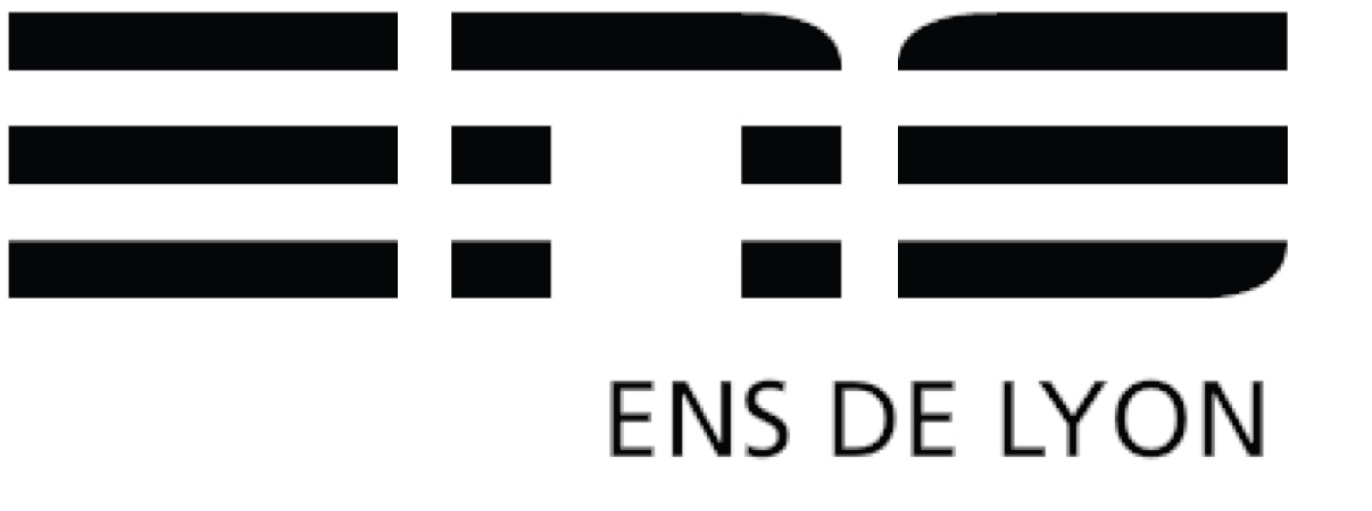
\includegraphics[height=1.9cm]{logo-ens.jpg} \hfill 
\includegraphics[height=2cm]{logo_lyon1.jpg} \hfill 
\includegraphics[height=2cm]{logo_univ_lyon.jpg}



Master Sciences de la matière
\hfill
Projet de Transition de phase 

\textit{École Normale Supérieure de Lyon}
\hfill
BUNEL Félix et VERGNET Hadrien

\textit{Université Claude Bernard Lyon 1}
\hfill
M2 Physique 2015-2016
\vspace{0.5cm}

\hrulefill
\vspace{-0.6cm}

\hrulefill


\begin{center}\bfseries
\vspace{0.3cm}
\begin{huge}
    Exploration numérique de la transition isotrope-nématique
\end{huge}
\end{center}

\hrulefill
\vspace{-0.6cm}

\hrulefill


\begin{center}
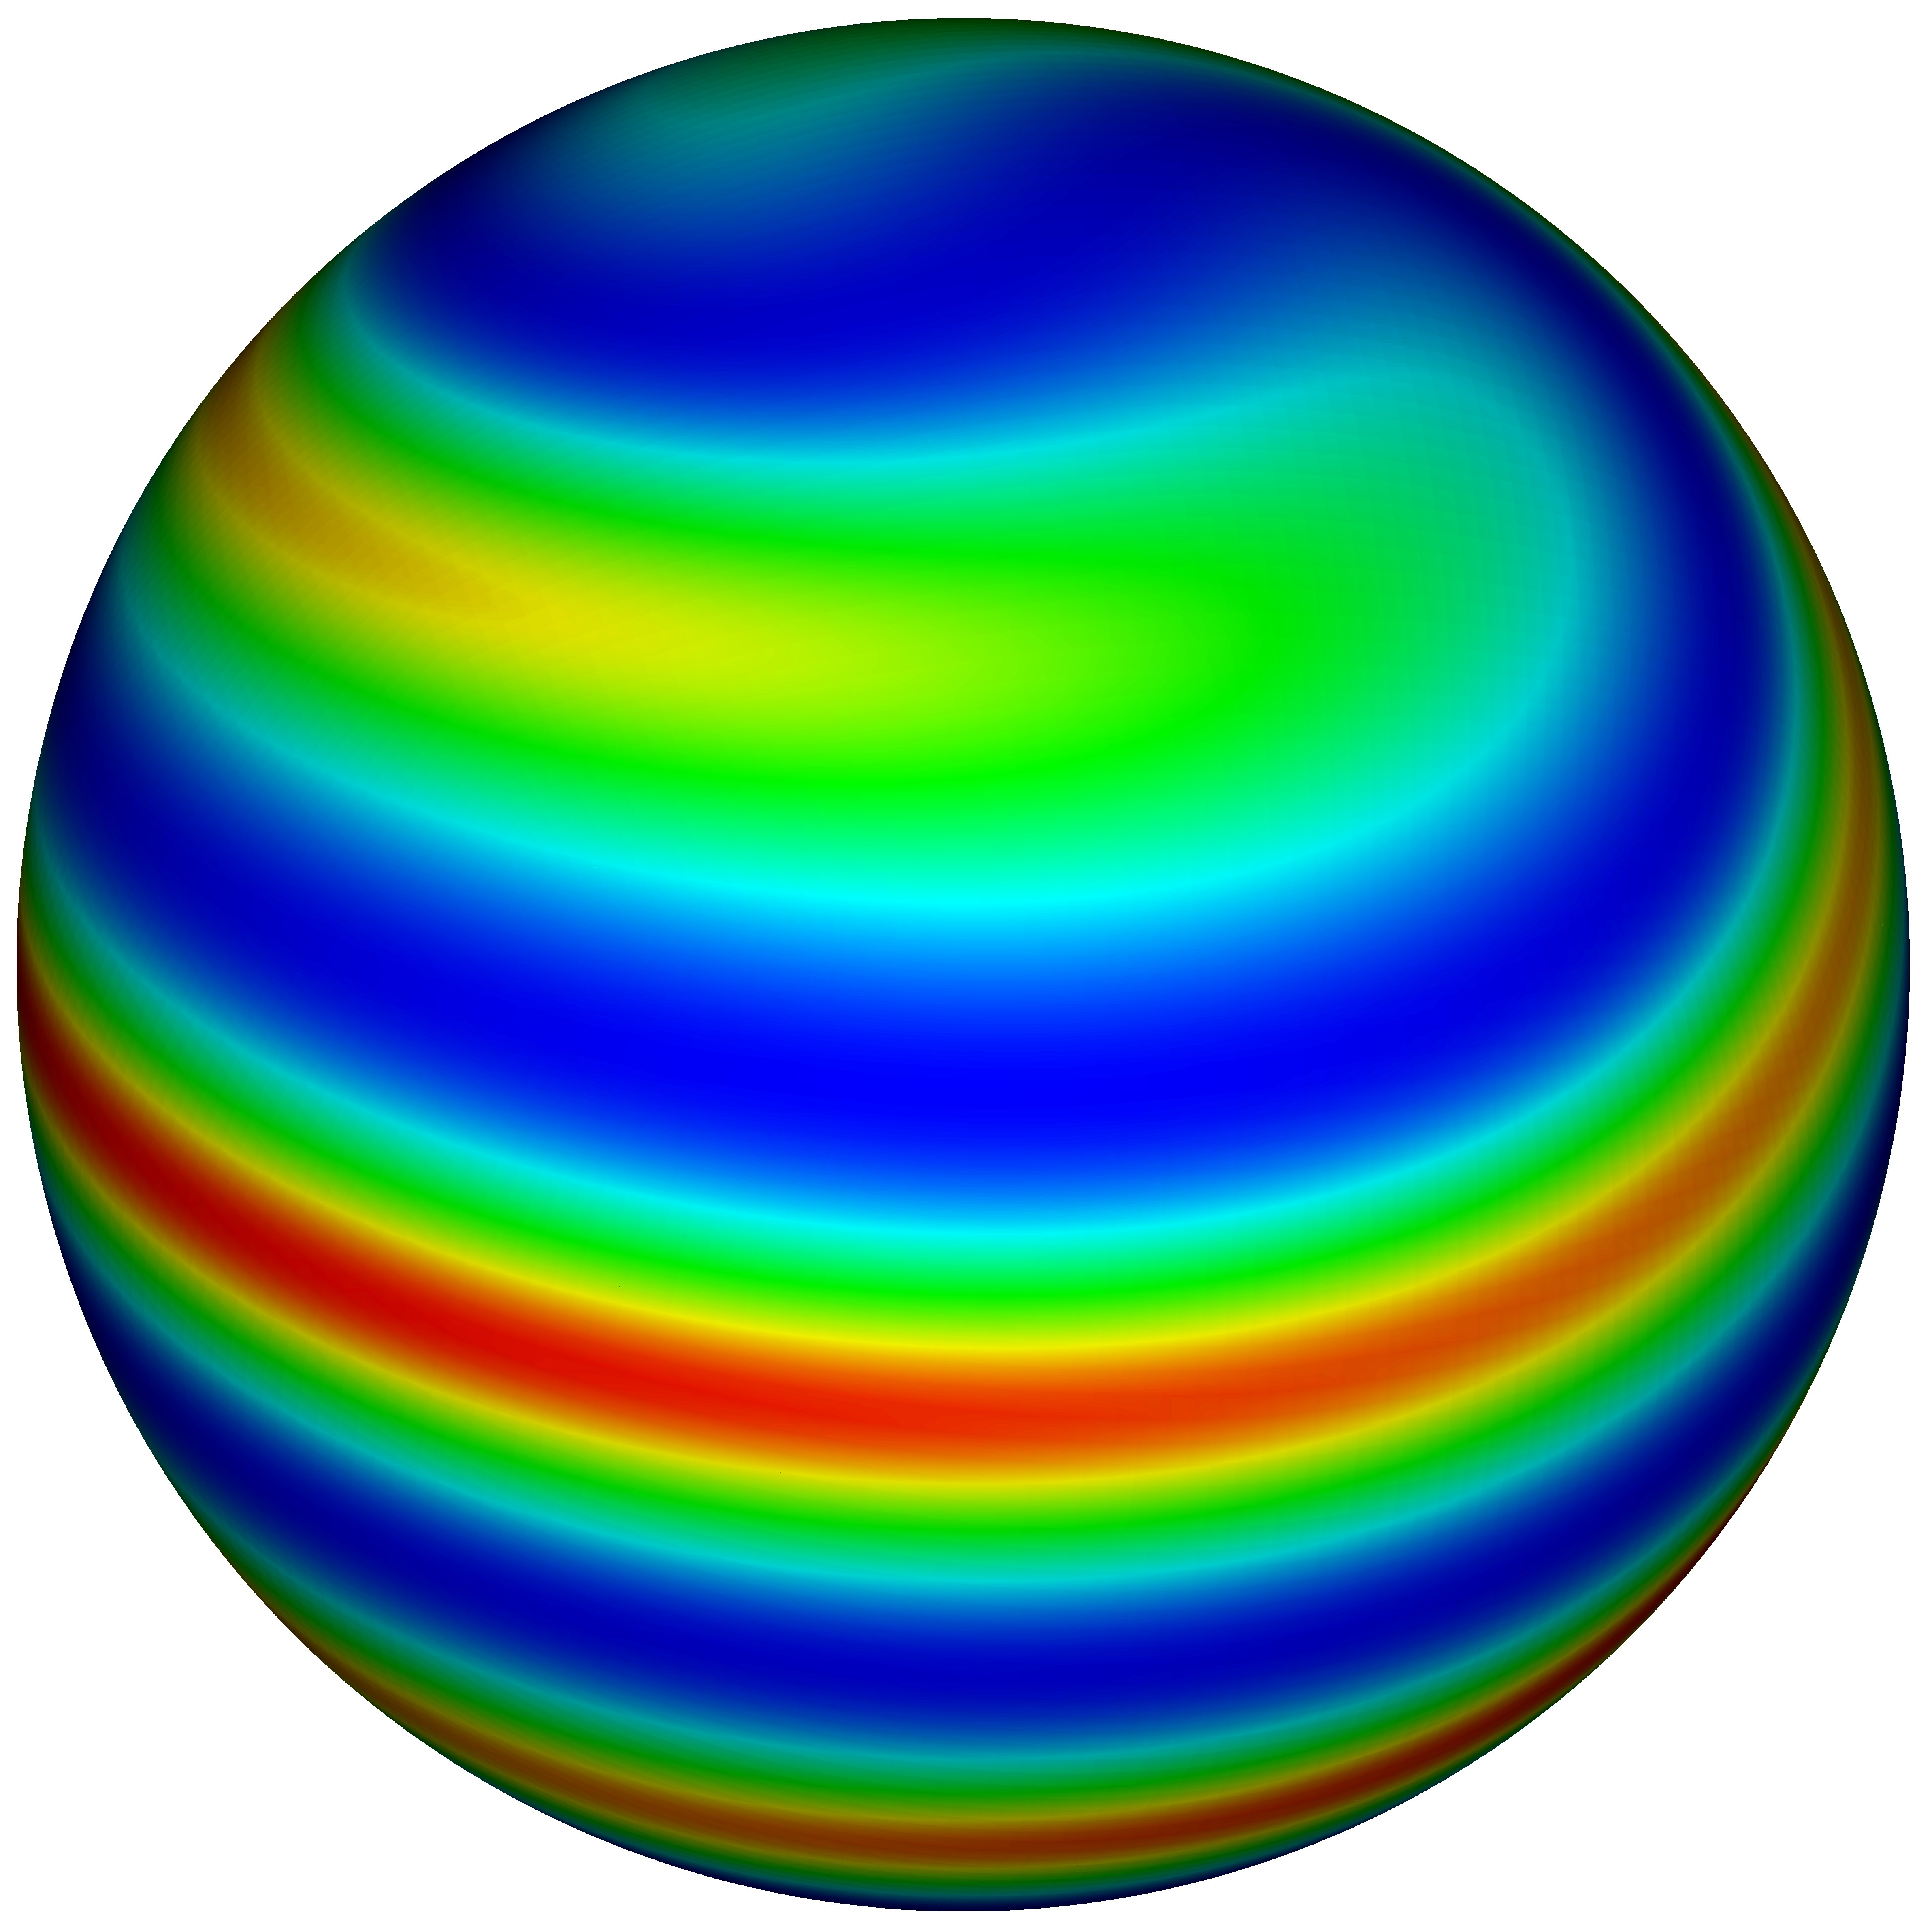
\includegraphics[height=6cm]{figures/front_simu.jpg} 
\end{center} 


\textbf{Résumé :} 
\vspace{0.3cm}

\textbf{Mots clefs :} cristaux liquides, nématique, Monte-Carlo.
\vspace{0.3cm}


\end{titlepage}

\newpage

\renewcommand\thepage{}

\section*{Remerciements}




\tableofcontents


\newpage
\renewcommand\thepage{\arabic{page}}
\setcounter{page}{1}


\definecolor{linkcolor}{rgb}{0,0,1}

%%%%%%%%%%%%%%%%%%%%%%%%%%%%%%%%%%%%%%%%%%%%%%%%%%%%%%%%%%%%%%%%%%%%%%%%%%%%%%%%%%%%%%%%
%%%%%%%%%%%%%%%%%%%%%%%%%%%%%%%%%%%%%%%%%%%%%%%%%%%%%%%%%%%%%%%%%%%%%%%%%%%%%%%%%%%%%%%%
\section*{Introduction}
%%%%%%%%%%%%%%%%%%%%%%%%%%%%%%%%%%%%%%%%%%%%%%%%%%%%%%%%%%%%%%%%%%%%%%%%%%%%%%%%%%%%%%%%
%%%%%%%%%%%%%%%%%%%%%%%%%%%%%%%%%%%%%%%%%%%%%%%%%%%%%%%%%%%%%%%%%%%%%%%%%%%%%%%%%%%%%%%%
\addcontentsline{toc}{section}{Introduction}
Le domaine des cristaux liquides a subi une importante expansion durant tout le 20\up{ème} siècle et est encore aujourd'hui un domaine actif de la recherche en physique. 
L'intérêt pour ces milieux intermédiaires entre cristaux et liquides provient entre autres de leurs applications industrielles en matière d'afficheurs (Figure \ref{lcd}).

\begin{figure}[h]
    \centering	    
	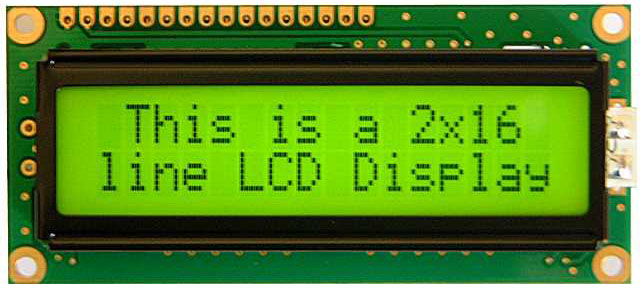
\includegraphics[height=3cm]{figures/lcd.jpg}
    \caption{Un écran à cristaux liquides}
    	\label{lcd} 
\end{figure}

Le nom cristal liquide regroupe les molécules ou mélange de molécules possédant une mésophase, c'est à dire une phase partiellement structurée, intermédiaire entre les phases liquide et cristalline.
Dans ce rapport, on s'intéressera au cas particulier de la phase nématique qui emprunte aux liquides l'invariance par translation, mais brise partiellement la symétrie par rotation.
Dans cette phase, les molécules s'organisent en effet pour avoir une orientation identique en moyenne (Figure \ref{nematic_phase}).

\begin{figure}[h]
    \center
    \begin{tikzpicture}[radius=0.1]
	\draw [->, >=stealth] (-1,2) -- (7.5,2) node[right]{T};
	\draw (3.35,1.9) -- (3.35,2.1) node[above]{$T^\star$};
	\draw [dashed] (3.35,2) -- (3.35,-1);

	\pgfmathsetseed{100}
	\pgfmathsetmacro{\xi}{0};
	\pgfmathsetmacro{\yi}{0};
	\foreach \i in {0,...,3}{
		\foreach \j in {0,...,2}{
			\pgfmathsetmacro{\x}{\xi+\i*0.6+0.04*rand};
			\pgfmathsetmacro{\y}{\yi+\j*0.7+0.1*rand};
			\pgfmathsetmacro{\angle}{rand*15};
			\drawZnema{\x}{\y}{\angle};
		}
	}
	\foreach \i in {0,...,3}{
		\foreach \j in {0,...,1}{
			\pgfmathsetmacro{\x}{\xi+0.3+\i*0.6+0.04*rand};
			\pgfmathsetmacro{\y}{\yi+0.35+\j*0.7+0.1*rand};
			\pgfmathsetmacro{\angle}{rand*15};
			\drawZnema{\x}{\y}{\angle};
		}
	}
	\draw [->,>=stealth] (0.5,-0.5) -- (1.5,-0.5);

	\pgfmathsetseed{79}
	\pgfmathsetmacro{\xi}{4.5};
	\pgfmathsetmacro{\yi}{0};
	\foreach \i in {0,...,3}{
		\foreach \j in {0,...,2}{
			\pgfmathsetmacro{\x}{\xi+\i*0.6+0.04*rand};
			\pgfmathsetmacro{\y}{\yi+\j*0.7+0.1*rand};
			\pgfmathsetmacro{\angle}{rand*180};
			\drawZnema{\x}{\y}{\angle};
		}
	}
	\foreach \i in {0,...,3}{
		\foreach \j in {0,...,1}{
			\pgfmathsetmacro{\x}{\xi+0.3+\i*0.6+0.04*rand};
			\pgfmathsetmacro{\y}{\yi+0.35+\j*0.7+0.1*rand};
			\pgfmathsetmacro{\angle}{rand*180};
			\drawZnema{\x}{\y}{\angle};
		}
	}


	\draw (1,-0.9) node[below]{\small phase nématique};
	\draw (5.75,-0.9) node[below]{\small phase isotrope};
\end{tikzpicture}

    \caption{Les cristaux liquides peuvent être représentées par un ensemble d'ellipsoïdes allongés dans une direction.
    Malgré les positions aléatoires des molécules, il existe un comportement collectif orientationnel : les molécules ont tendance à s'orienter dans la même direction en moyenne. }
    \label{nematic_phase}
\end{figure}

L'objectif de ce projet a été d'étudier par des méthodes numériques la transition de phase nématique-isotrope.
Ce rapport présente dans une première partie le modèle ainsi que les outils numériques utilisés. 
Une deuxième partie présentera les résultats obtenus sur la transition observée.
Enfin, une dernière partie étudiera l'influence d'un champ électrique sur cette transition.

\newpage
%%%%%%%%%%%%%%%%%%%%%%%%%%%%%%%%%%%%%%%%%%%%%%%%%%%%%%%%%%%%%%%%%%%%%%%%%%%%%%%%%%%%%%%%
%%%%%%%%%%%%%%%%%%%%%%%%%%%%%%%%%%%%%%%%%%%%%%%%%%%%%%%%%%%%%%%%%%%%%%%%%%%%%%%%%%%%%%%%
\section{Méthodes numériques}
%%%%%%%%%%%%%%%%%%%%%%%%%%%%%%%%%%%%%%%%%%%%%%%%%%%%%%%%%%%%%%%%%%%%%%%%%%%%%%%%%%%%%%%%
%%%%%%%%%%%%%%%%%%%%%%%%%%%%%%%%%%%%%%%%%%%%%%%%%%%%%%%%%%%%%%%%%%%%%%%%%%%%%%%%%%%%%%%%

\subsection{Modèle de Lebwohl-Lasher}
Le modèle de Lebwohl-Lasher \cite{model} est en quelque sorte l'analogue pour la transition nématique-isotrope du modèle d'Ising. Comme pour ce dernier, il permet d'obtenir des résultats très satisfaisant malgré sa simplicité.\medskip

\begin{figure}[h]
    \center
    \begin{tikzpicture}

    \pgfmathsetseed{1}
    

    \foreach \i in {0,...,5}{
        \pgfmathsetmacro{\x}{\i*0.7};
        \draw (\x,0) -- (\x,0.7*5);
        \draw (0,\x) -- (0.7*5,\x);
    }

    \foreach \i in {0,...,5}{
    \pgfmathsetmacro{\x}{\i*0.7};
        \foreach \j in {0,1,5}{
            
            \pgfmathsetmacro{\y}{\j*0.7};
            \pgfmathsetmacro{\angle}{rand*60};
            \pgfmathsetmacro{\size}{0.3};
            \drawNema{\x}{\y}{\angle}{\size};
        }
    }

    \foreach \j in {4,2,3}{
        \pgfmathsetmacro{\y}{\j*0.7};
        \foreach \i in {0,4,5}{
            \pgfmathsetmacro{\x}{\i*0.7};
            \pgfmathsetmacro{\angle}{rand*60};
            \pgfmathsetmacro{\size}{0.3};
            \drawNema{\x}{\y}{\angle}{\size};
        }
    }


    \pgfmathsetmacro{\xc}{2*0.7};
    \pgfmathsetmacro{\yc}{3*0.7};
    \pgfmathsetmacro{\anglec}{rand*60};
    \pgfmathsetmacro{\sizec}{0.3};

    \pgfmathsetmacro{\xul}{1*0.7};
    \pgfmathsetmacro{\yul}{4*0.7};
    \pgfmathsetmacro{\angleul}{rand*60};
    \pgfmathsetmacro{\sizeul}{0.3};

    \pgfmathsetmacro{\xum}{2*0.7};
    \pgfmathsetmacro{\yum}{4*0.7};
    \pgfmathsetmacro{\angleum}{rand*60};
    \pgfmathsetmacro{\sizeum}{0.3};

    \pgfmathsetmacro{\xur}{3*0.7};
    \pgfmathsetmacro{\yur}{4*0.7};
    \pgfmathsetmacro{\angleur}{rand*60};
    \pgfmathsetmacro{\sizeur}{0.3};

    \pgfmathsetmacro{\xmr}{1*0.7};
    \pgfmathsetmacro{\ymr}{3*0.7};
    \pgfmathsetmacro{\anglemr}{rand*60};
    \pgfmathsetmacro{\sizemr}{0.3};

    \pgfmathsetmacro{\xml}{3*0.7};
    \pgfmathsetmacro{\yml}{3*0.7};
    \pgfmathsetmacro{\angleml}{rand*60};
    \pgfmathsetmacro{\sizeml}{0.3};

    \pgfmathsetmacro{\xdl}{1*0.7};
    \pgfmathsetmacro{\ydl}{2*0.7};
    \pgfmathsetmacro{\angledl}{rand*60};
    \pgfmathsetmacro{\sizedl}{0.3};

    \pgfmathsetmacro{\xdr}{3*0.7};
    \pgfmathsetmacro{\ydr}{2*0.7};
    \pgfmathsetmacro{\angledr}{rand*60};
    \pgfmathsetmacro{\sizedr}{0.3};

    \pgfmathsetmacro{\xdm}{2*0.7};
    \pgfmathsetmacro{\ydm}{2*0.7};
    \pgfmathsetmacro{\angledm}{rand*60};
    \pgfmathsetmacro{\sizedm}{0.3};

            \drawNema{\xul}{\yul}{\angleul}{\sizeul};
            \drawNema{\xum}{\yum}{\angleum}{\sizeum};
            \drawNema{\xur}{\yur}{\angleur}{\sizeur};

            \drawNema{\xml}{\yml}{\angleml}{\sizeml};
            \drawNema{\xmr}{\ymr}{\anglemr}{\sizemr};

            \drawNema{\xdr}{\ydr}{\angledr}{\sizedr};
            \drawNema{\xdl}{\ydl}{\angledl}{\sizedl};
            \drawNema{\xdm}{\ydm}{\angledm}{\sizedm};

            \drawNema{\xc}{\yc}{\anglec}{\sizec};
    


\end{tikzpicture}

    \caption{Représentation à deux dimensions du modèle de Lebwohl-Lasher.}
    \label{lebwohl}
\end{figure}


Dans ce modèle, les molécules de cristal liquides sont représentés uniquement par leur direction et occupent des positions fixes sur les sites d'un réseau cubique.
Les différents sites du réseau interagissent uniquement entre plus proches voisins par l'intermédiaire d'un potentiel de la forme :
\begin{equation}
E_{i,j} = - \epsilon\ \frac{3\cos^2\theta_{i,j}-1}{2}
\end{equation}
où $\epsilon$ est une constante positive et $\theta_{i,j}$ est l'angle entre les deux molécules voisines. 
Cette énergie est minimale lorsque les molécules sont parfaitement alignées : si $\theta_{i,j} = 0$ alors $E_{i,j} = - \epsilon$. Elle est maximale lorsque les molécules ont des directions orthogonales : si $\theta_{i,j} = \pi/2$ alors $E_{i,j} = \epsilon/2$.
Ces interactions auront donc tendance à favoriser les configurations ou les molécules pointent toutes dans la même direction.\medskip

On comprend alors assez bien pourquoi ce système subit une transition de phase. Les deux énergies intervenant dans ce système sont celles de l'interaction entre les molécules et celle de l'agitation thermique dont les échelles sont respectivement $\epsilon$ et $k_B T$.
A haute température, l'agitation thermique prédomine et l'orientation des molécules est aléatoire. A basse température, l'énergie d'interaction entre les sites est la plus importante et les molécules privilégient une direction commune.\medskip

Pour toute notre étude, des conditions aux limites périodiques ont été imposées mais d'autres conditions sont également possibles. Des travaux récents \cite{confined} ont par exemple utilisé une énergie à la surface de la même forme que le potentiel d'interaction pour simuler une cellule avec un ancrage aux parois. 

%L'énergie totale du système qui découle de cette interaction s'écrit simplement comme une somme sur les paires de plus proches voisins :
%\begin{equation}
%E = - \epsilon\ \sum_{<i,j>} \frac{3\cos^2\theta_{i,j}-1}{2}
%\end{equation}

\subsection{Paramètre d'ordre}

\subsection{Algorithme Monte-Carlo}

L'idée de base derrière les algorithmes de type Monte-Carlo est de remplacer le calcul d'intégrales sur l'espace des phases par des moyennes sur une marche aléatoires. L'évolution Monte-Carlo de notre système utilise l'algorithme proposé par Metropolis et al \cite{metropolis} qui consiste à réaliser une série de mouvement aléatoire et d'accepter ces changements avec une probabilité en fonction de la variation d'énergie.\medskip

Plus précisément, on commence par sélectionner un site du réseau. Ensuite, une nouvelle direction de la molécule est tirée aléatoirement. Si ce changement diminue l'énergie totale du système, le changement est accepté. Sinon, le changement est accepté avec une probabilité proportionnel au poids de Boltzmann de la variation d'énergie $\Delta E$ :

\begin{equation}
p = e^{-\Delta E / k_B T}
\label{boltzmannprob}
\end{equation}
Il est important de noter que cette formule n'est valable que lorsque toute les directions ont la même probabilité d'être tirées. Sinon, il faut ajouter un facteur multiplicatif correspondant au rapport des probabilités de tirer les directions de départ et d'arrivée.
\medskip

Il est possible de montrer qu'un grand nombre de répétition de ces mouvements permet d'obtenir la configuration d'équilibre du système. Des moyennes statistiques pour les quantités d'intérêts peuvent ensuite être calculés sur les micro-états générés par l'algorithme une fois l'équilibre atteint.

\subsection{Implémentation}
Les simulations reportées dans ce rapport ont toutes été réalisées sur un réseau cubique de taille $30\times 30\times 30$ avec des conditions aux limites périodiques. 

\subsubsection{Équiprobabilité des directions}
Pour chaque site du réseau, l'orientation de la molécule est stockée en tant que $\cos \theta$ et $\phi$ où $\theta$ et $\phi$ sont respectivement les angles polaires et azimutales. Utiliser ces variables plutôt que simplement $\theta$ et $\phi$ est nécessaire à l'équiprobabilité des directions. En effet, si l'on tire au hasard un $\theta$ et un $\phi$, la probabilité d'obtenir une direction proche du pole est plus importante. Cette anisotropie disparaît lorsque l'on tire un $\cos \theta$ et un $\phi$. Cela se comprend assez bien en se rappelant que l'élément de surface en sphérique s'écrit $d\theta\, \sin \theta d\phi = d\text{cos}\,\theta\, d\phi$.

\subsubsection{Ratio d'acceptation}
Le fait de choisir une nouvelle direction sur l'ensemble de la sphère unité pose certains problèmes. En effet, si l'on part de l'état fondamental où toute les molécules sont alignées, une grande partie des mouvements tentées seront refusées quelque soit la température car ils augmentent fortement l'énergie du système. Cet effet se maintient au delà de la température de transition à laquelle le ratio d'acceptation n'est encore que de   30$\%$. Par conséquent, très peu de micro-états différents sont observées et les moyennes calculées ne rendent alors pas bien compte de la physique du système.

Afin d'obtenir de meilleurs résultats et de faire bon usage du temps de calcul, il est possible d'implémenter des méthodes pour obtenir un ratio d'acceptation de $1/2$. 

Restricting the random steps to be very small would result on average in a high acceptance ratio since
trial moves that result in a large unfavorable energy shift are unlikely. Because each cycle only results in
slight changes, the model will equilibrate slowly. On the other hand, if we allow for the full possible
random step ranges, each trial move dramatically changes the local energy. Significant movement often
disturbs the local ordering and results in a sizable increase in energy. As a consequence, these moves
are unlikely to be accepted and computation time is wasted generating rejected moves; hence the need
to generate moves that are likely to be both accepted and to meaningfully move the system towards
equilibrium.


\subsubsection{Déroulement d'une simulation} 
Les simulations sont commencées depuis l'état fondamental où toutes les molécules sont alignées. Lorsque l'on démarre la simulation, les molécules sont bougées les unes après les autres en utilisant l'algorithme de Monte-Carlo. On nomme un cycle une suite de $30\times 30\times 30$ mouvements. Durant un cycle, toutes les molécules du réseau sont bougées exactement une fois mais dans un ordre aléatoire. Une telle procédure assure que toutes les molécules ont la même chance d'être bougée en réduisant les irrégularités dues à un tirage totalement aléatoire \cite{fabbri}. 
\medskip

Pour chaque température, au minimum 1000 cycles sont calculées pour faire évoluer le système vers la configuration d'équilibre. Les variations de l'énergie et du paramètre d'ordre permettent de vérifier que le système est bien à l'équilibre. Ensuite, jusqu'à 25 000 cycles sont réalisées afin de calculer les quantités d'intérêts.

\subsubsection{Langage de programmation}
Une première version du code a été implémentée en \texttt{Python} et a permis d'obtenir simplement des résultats. L'existence de bibliothèque comme \texttt{Numpy} permet d'obtenir un code fonctionnant de manière rapide et intuitive. Cependant, \texttt{Python} n'est pas adapté à des algorithmes de type Monte-Carlo qui consiste en de longues itérations. Ainsi, une seconde version du code plus performante a été implémentée en \CC. Ce dernier tourne en moyenne 40 fois plus vite que son homologue en \texttt{Python} ce qui a permis de réaliser de plus grosse simulations. L'utilisation des ressources du Centre Blaise Pascal a également été d'une grande aide pour réaliser des simulations sur une longue durée. Les deux versions du code sont disponibles en libre accès sur la plateforme github \cite{github}.
\newpage
%%%%%%%%%%%%%%%%%%%%%%%%%%%%%%%%%%%%%%%%%%%%%%%%%%%%%%%%%%%%%%%%%%%%%%%%%%%%%%%%%%%%%%%%
%%%%%%%%%%%%%%%%%%%%%%%%%%%%%%%%%%%%%%%%%%%%%%%%%%%%%%%%%%%%%%%%%%%%%%%%%%%%%%%%%%%%%%%%
\section{Transition nématique-isotrope}
%%%%%%%%%%%%%%%%%%%%%%%%%%%%%%%%%%%%%%%%%%%%%%%%%%%%%%%%%%%%%%%%%%%%%%%%%%%%%%%%%%%%%%%%
%%%%%%%%%%%%%%%%%%%%%%%%%%%%%%%%%%%%%%%%%%%%%%%%%%%%%%%%%%%%%%%%%%%%%%%%%%%%%%%%%%%%%%%%




\newpage
%%%%%%%%%%%%%%%%%%%%%%%%%%%%%%%%%%%%%%%%%%%%%%%%%%%%%%%%%%%%%%%%%%%%%%%%%%%%%%%%%%%%%%%%
%%%%%%%%%%%%%%%%%%%%%%%%%%%%%%%%%%%%%%%%%%%%%%%%%%%%%%%%%%%%%%%%%%%%%%%%%%%%%%%%%%%%%%%%
\section{Influence d'un champ électrique}
%%%%%%%%%%%%%%%%%%%%%%%%%%%%%%%%%%%%%%%%%%%%%%%%%%%%%%%%%%%%%%%%%%%%%%%%%%%%%%%%%%%%%%%%
%%%%%%%%%%%%%%%%%%%%%%%%%%%%%%%%%%%%%%%%%%%%%%%%%%%%%%%%%%%%%%%%%%%%%%%%%%%%%%%%%%%%%%%%


\newpage
%%%%%%%%%%%%%%%%%%%%%%%%%%%%%%%%%%%%%%%%%%%%%%%%%%%%%%%%%%%%%%%%%%%%%%%%%%%%%%%%%%%%%%%%
%%%%%%%%%%%%%%%%%%%%%%%%%%%%%%%%%%%%%%%%%%%%%%%%%%%%%%%%%%%%%%%%%%%%%%%%%%%%%%%%%%%%%%%%
\section*{Conclusion}
%%%%%%%%%%%%%%%%%%%%%%%%%%%%%%%%%%%%%%%%%%%%%%%%%%%%%%%%%%%%%%%%%%%%%%%%%%%%%%%%%%%%%%%%
%%%%%%%%%%%%%%%%%%%%%%%%%%%%%%%%%%%%%%%%%%%%%%%%%%%%%%%%%%%%%%%%%%%%%%%%%%%%%%%%%%%%%%%%
\addcontentsline{toc}{section}{Conclusion}


\newpage
%%%%%%%%%%%%%%%%%%%%%%%%%%%%%%%%%%%%%%%%%%%%%%%%%%%%%%%%%%%%%%%%%%%%%%%%%%%%%%%%%%%%%%%
%%%%%%%%%%%%%%%%%%%%%%%%%%%%%%%%%%%%%%%%%%%%%%%%%%%%%%%%%%%%%%%%%%%%%%%%%%%%%%%%%%%%%%%
\appendix
%%%%%%%%%%%%%%%%%%%%%%%%%%%%%%%%%%%%%%%%%%%%%%%%%%%%%%%%%%%%%%%%%%%%%%%%%%%%%%%%%%%%%%%
%%%%%%%%%%%%%%%%%%%%%%%%%%%%%%%%%%%%%%%%%%%%%%%%%%%%%%%%%%%%%%%%%%%%%%%%%%%%%%%%%%%%%%%
\section{Première annexe} \label{annexe_fonctionnelles}


\newpage
\bibliographystyle{unsrt}
\bibliography{biblio} 
\addcontentsline{toc}{section}{Références} 


\end{document}
